\documentclass[
  convert={
    command={\g_standalone_gs_command\space -dSAFER -dBATCH -dNOPAUSE -sDEVICE=png16m -r300 -sOutputFile=\OutputFile\space \InputFile}
  },
  border=5mm
]{standalone}
\usepackage{amsmath}
\usepackage{pgfplots}
\pgfplotsset{compat=1.18}
\usetikzlibrary{arrows.meta, fit, backgrounds, calc}

% ---- colours -----------------------------------------------------------
\definecolor{ink}{HTML}{1F2937}
\definecolor{ink2}{HTML}{4B5563}
\definecolor{muted}{HTML}{9CA3AF}
\definecolor{trunkfill}{HTML}{EEF4FB}
\definecolor{trunkline}{HTML}{2A78D6}
\definecolor{detfill}{HTML}{F3F4F6}
\definecolor{detline}{HTML}{4B5563}
\definecolor{luckfill}{HTML}{FDF1F5}
\definecolor{luckline}{HTML}{D6336C}
\definecolor{expfill}{HTML}{FFF7E8}
\definecolor{expline}{HTML}{C2410C}
\definecolor{endfill}{HTML}{EEF8F1}
\definecolor{endline}{HTML}{2F855A}

% ---- styles ------------------------------------------------------------
\tikzset{
  base/.style = {rounded corners=3pt, line width=0.7pt, inner sep=5pt,
    font=\small, text=ink, align=left,
    execute at begin node={\hyphenpenalty=10000\exhyphenpenalty=10000
      \setlength{\parskip}{2pt}}},
  trunk/.style = {base, draw=trunkline, fill=trunkfill},
  dstep/.style = {base, draw=detline, fill=white, text width=6.75cm},
  lstep/.style = {base, draw=luckline, fill=white, text width=6.75cm},
  group/.style = {rounded corners=7pt, line width=0.9pt, dashed,
    inner sep=0pt},
  gtitle/.style = {font=\small, text=ink, align=left, inner sep=0pt,
    text width=7.3cm, anchor=north west},
  arrow/.style = {-{Stealth[length=2.4mm]}, line width=0.8pt, draw=ink2},
  line/.style = {line width=0.8pt, draw=ink2},
  note/.style = {font=\footnotesize, text=ink2, align=left, inner sep=1pt}
}
\newcommand{\ttl}[1]{\textbf{#1}\par}
\newcommand{\eq}[1]{\par{\centering$\displaystyle #1$\par}}
\newenvironment{tight}{\begin{list}{\textbullet}{%
    \setlength{\leftmargin}{0.9em}\setlength{\labelwidth}{0.6em}%
    \setlength{\labelsep}{0.3em}\setlength{\itemsep}{2pt}%
    \setlength{\parsep}{0pt}\setlength{\topsep}{2pt}}}{\end{list}}

% ---- plot styles -------------------------------------------------------
\pgfplotsset{
  demo/.style = {scale only axis, width=5.2cm, axis line style={ink2},
    tick style={ink2}, ticklabel style={font=\scriptsize, text=ink2},
    label style={font=\footnotesize, text=ink},
    every axis plot/.append style={line join=round}},
  branch/.style = {trunkline, line width=1.1pt, mark=none},
  drop/.style = {trunkline, dotted, line width=0.8pt, mark=none},
  run/.style = {line width=0.7pt, mark=none}
}

\begin{document}
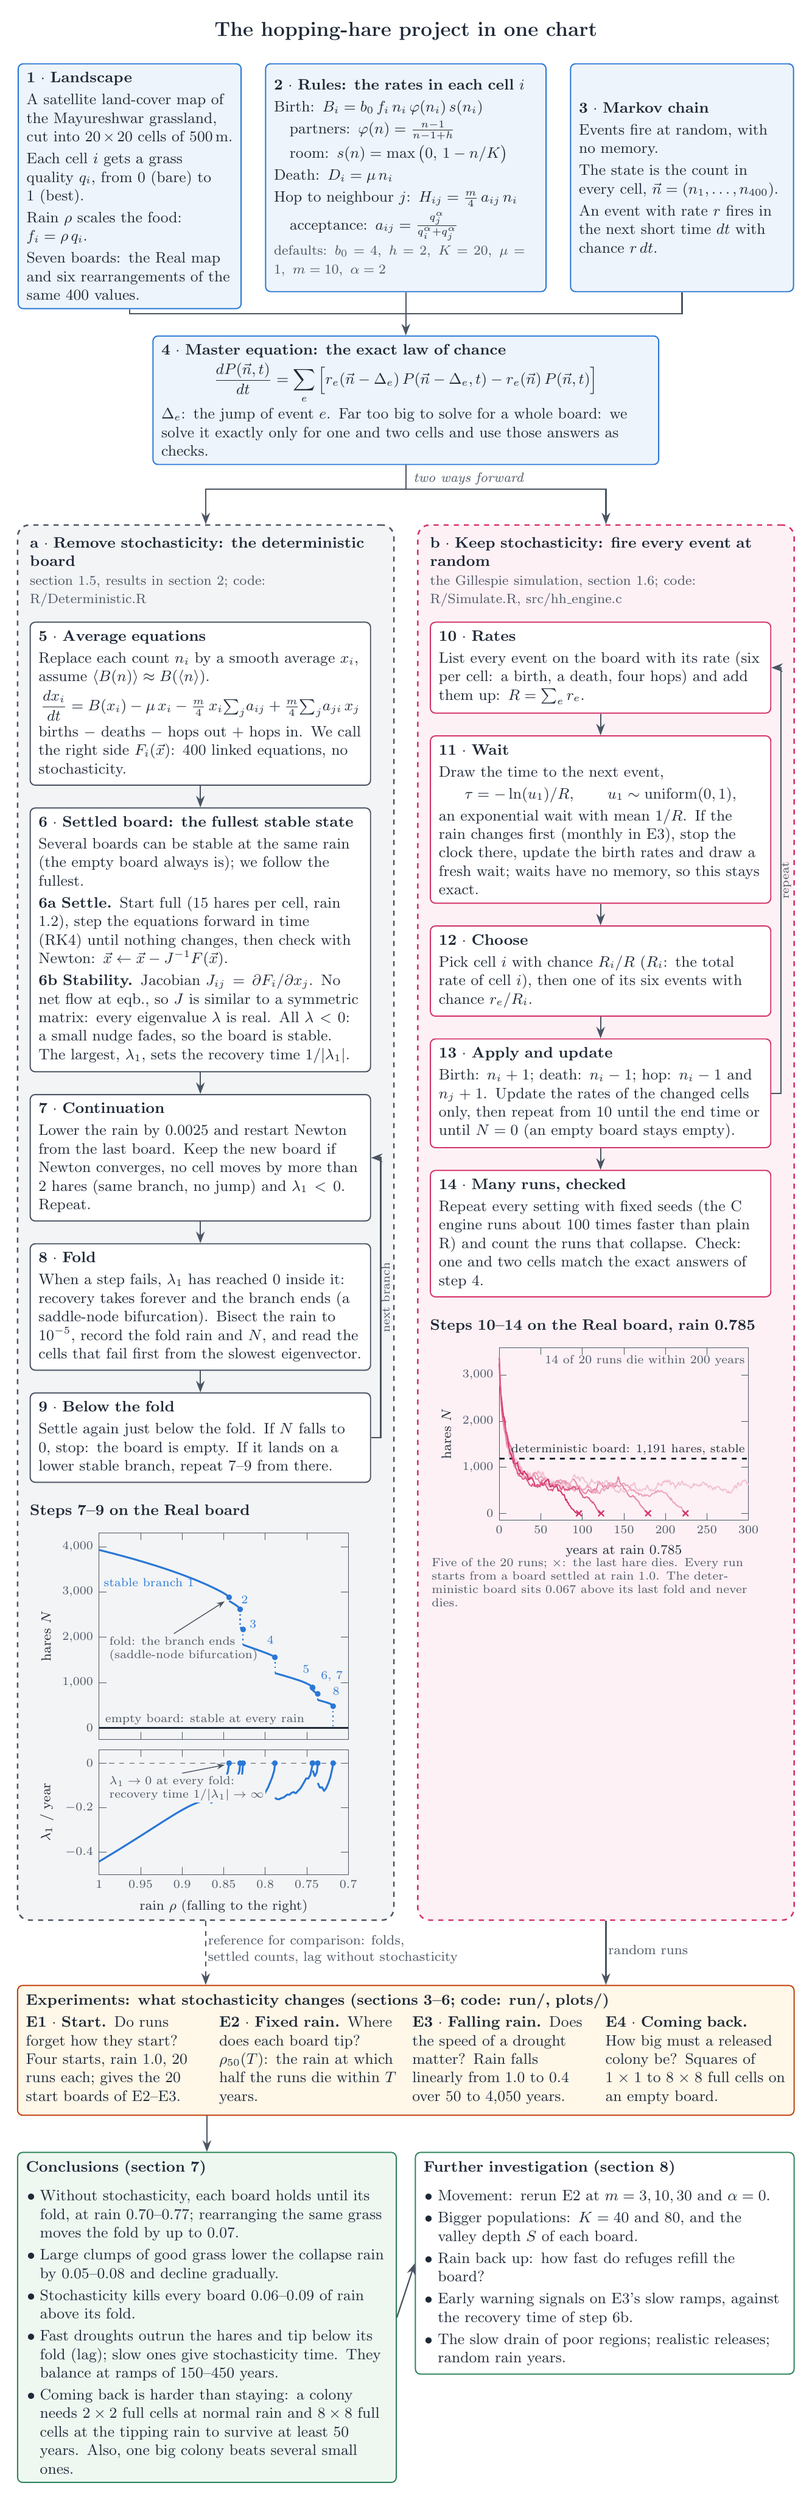
\begin{tikzpicture}

% ======================================================================
% Title
% ======================================================================
\node[font=\large\bfseries, text=ink, anchor=south] at (8.1, 0.35)
  {The hopping-hare project in one chart};

% ======================================================================
% Trunk: 1, 2, 3 side by side, merging into 4
% ======================================================================
\node[trunk, text width=4.3cm, minimum height=4.75cm, anchor=north west]
  (s1) at (0, 0) {%
  \ttl{1 $\cdot$ Landscape}
  A satellite land-cover map of the Mayureshwar grassland, cut into
  $20\times20$ cells of 500\,m.\par
  Each cell $i$ gets a grass quality $q_i$, from 0 (bare) to 1 (best).\par
  Rain $\rho$ scales the food: \\ $f_i=\rho\,q_i$.\par
  Seven boards: the Real map and six rearrangements of the same 400
  values.};

\node[trunk, text width=5.5cm, minimum height=4.75cm, anchor=north]
  (s2) at (8.1, 0) {%
  \ttl{2 $\cdot$ Rules: the rates in each cell $i$}
  Birth: $B_i=b_0\,f_i\,n_i\,\varphi(n_i)\,s(n_i)$\par
  \quad partners: $\varphi(n)=\frac{n-1}{n-1+h}$\par
  \quad room: $s(n)=\max\big(0,\,1-n/K\big)$\par
  Death: $D_i=\mu\,n_i$\par
  Hop to neighbour $j$: $H_{ij}=\frac{m}{4}\,a_{ij}\,n_i$\par
  \quad acceptance: $a_{ij}=\frac{q_j^{\alpha}}{q_i^{\alpha}+q_j^{\alpha}}$
  \par
  {\color{ink2}\footnotesize defaults: $b_0=4,\ h=2,\ K=20,\ \mu=1,\
  m=10,\ \alpha=2$}};

\node[trunk, text width=4.3cm, minimum height=4.75cm, anchor=north east]
  (s3) at (16.2, 0) {%
  \ttl{3 $\cdot$ Markov chain}
  Events fire at random, with no memory.\par
  The state is the count in every cell, $\vec n=(n_1,\dots,n_{400})$.\par
  An event with rate $r$ fires in the next short time $dt$ with chance
  $r\,dt$.};

\coordinate (bus) at ($(s2.south)+(0,-0.45)$);
\node[trunk, text width=10.2cm, anchor=north] (s4)
  at ($(bus)+(0,-0.45)$) {%
  \ttl{4 $\cdot$ Master equation: the exact law of chance}
  \eq{\frac{dP(\vec n,t)}{dt}=\sum_e\Big[r_e(\vec n-\Delta_e)\,
    P(\vec n-\Delta_e,t)-r_e(\vec n)\,P(\vec n,t)\Big]}
  $\Delta_e$: the jump of event $e$. Far too big to solve for a whole
  board: we solve it exactly only for one and two cells and use those answers as checks.};

\draw[line] (s1.south) |- (bus);
\draw[line] (s3.south) |- (bus);
\draw[line] (s2.south) -- (bus);
\draw[arrow] (bus) -- (s4.north);

\coordinate (split) at ($(s4.south)+(0,-0.5)$);
\coordinate (gtop) at ($(split)+(0,-0.75)$);
\node[note, anchor=south west, font=\footnotesize\itshape]
  at ($(split)+(0.12,0.05)$) {two ways forward};

% ======================================================================
% Branch a: remove stochasticity, the deterministic board
% ======================================================================
\node[gtitle] (ta) at ($(0.25,0 |- gtop)+(0,-0.25)$) {%
  \textbf{a $\cdot$ Remove stochasticity: the deterministic board}\\
  {\color{ink2}\footnotesize section 1.5, results in section 2;
  code: R/Deterministic.R}};

\node[dstep, anchor=north west] (s5) at ($(ta.south west)+(0,-0.3)$) {%
  \ttl{5 $\cdot$ Average equations}
  Replace each count $n_i$ by a smooth average $x_i$,\\
  assume $\langle B(n)\rangle\approx B(\langle n\rangle)$.
  \eq{\frac{dx_i}{dt}=B(x_i)-\mu\,x_i
    -\tfrac{m}{4}\,x_i{\textstyle\sum_j}a_{ij}
    +\tfrac{m}{4}{\textstyle\sum_j}a_{ji}\,x_j}
  births $-$ deaths $-$ hops out $+$ hops in. We call the right side
  $F_i(\vec x)$: 400 linked equations, no stochasticity.};

\node[dstep, anchor=north west] (s6) at ($(s5.south west)+(0,-0.45)$) {%
  \ttl{6 $\cdot$ Settled board: the fullest stable state}
  Several boards can be stable at the same rain (the empty board always
  is); we follow the fullest.\par
  \textbf{6a Settle.} Start full (15 hares per cell, rain 1.2), step
  the equations forward in time (RK4) until nothing changes, then
  check with Newton: $\vec x\leftarrow\vec x-J^{-1}F(\vec x)$.\par
  \textbf{6b Stability.} Jacobian $J_{ij}=\partial F_i/\partial x_j$.
  No net flow at eqb., so $J$ is similar to a symmetric matrix:
  every eigenvalue $\lambda$ is real. All $\lambda<0$: a small nudge
  fades, so the board is stable. The largest, $\lambda_1$, sets the
  recovery time $1/|\lambda_1|$.};

\node[dstep, anchor=north west] (s7) at ($(s6.south west)+(0,-0.45)$) {%
  \ttl{7 $\cdot$ Continuation}
  Lower the rain by 0.0025 and restart Newton from the last board. Keep
  the new board if Newton converges, no cell moves by more than 2 hares
  (same branch, no jump) and $\lambda_1<0$. Repeat.};

\node[dstep, anchor=north west] (s8) at ($(s7.south west)+(0,-0.45)$) {%
  \ttl{8 $\cdot$ Fold}
  When a step fails, $\lambda_1$ has reached 0 inside it: recovery
  takes forever and the branch ends (a saddle-node bifurcation). Bisect
  the rain to $10^{-5}$, record the fold rain and $N$, and read the
  cells that fail first from the slowest eigenvector.};

\node[dstep, anchor=north west] (s9) at ($(s8.south west)+(0,-0.45)$) {%
  \ttl{9 $\cdot$ Below the fold}
  Settle again just below the fold. If $N$ falls to 0, stop: the board
  is empty. If it lands on a lower stable branch, repeat 7--9 from
  there.};

\foreach \a/\b in {s5/s6, s6/s7, s7/s8, s8/s9}
  \draw[arrow] (\a.south) -- (\b.north);
\draw[arrow] (s9.east) -- ++(0.2,0) |- (s7.east)
  node[pos=0.25, right=-1pt, note, rotate=90, anchor=north,
       font=\scriptsize] {next branch};

% ---- plot A: steps 7-9 on the Real board ------------------------------
\node[gtitle, text width=6.9cm] (pa) at ($(s9.south west)+(0,-0.45)$)
  {\textbf{Steps 7--9 on the Real board}};
\coordinate (pA0) at ($(pa.south west)+(1.45,-0.3)$);
\begin{axis}[demo, name=foldN, at={(pA0)},
    anchor=north west, height=4.3cm,
    xmin=0.70, xmax=1.0, x dir=reverse, ymin=-250, ymax=4300,
    xtick={0.7,0.75,...,1.0}, xticklabels={},
    ytick={0,1000,2000,3000,4000},
    ylabel={hares $N$}, clip=false]
    \addplot[branch] coordinates {(1.00000,3926) (0.99750,3915) (0.99500,3903) (0.99250,3892) (0.99000,3880) (0.98750,3868) (0.98500,3857) (0.98250,3845) (0.98000,3833) (0.97750,3820) (0.97500,3808) (0.97250,3796) (0.97000,3784) (0.96750,3771) (0.96500,3758) (0.96250,3746) (0.96000,3733) (0.95750,3720) (0.95500,3707) (0.95250,3693) (0.95000,3680) (0.94750,3667) (0.94500,3653) (0.94250,3639) (0.94000,3625) (0.93750,3611) (0.93500,3597) (0.93250,3583) (0.93000,3568) (0.92750,3554) (0.92500,3539) (0.92250,3524) (0.92000,3509) (0.91750,3493) (0.91500,3478) (0.91250,3462) (0.91000,3446) (0.90750,3430) (0.90500,3414) (0.90250,3397) (0.90000,3380) (0.89750,3363) (0.89500,3346) (0.89250,3328) (0.89000,3310) (0.88750,3292) (0.88500,3274) (0.88250,3255) (0.88000,3236) (0.87750,3216) (0.87500,3197) (0.87250,3177) (0.87000,3156) (0.86750,3135) (0.86500,3114) (0.86250,3092) (0.86000,3070) (0.85750,3047) (0.85500,3023) (0.85250,2999) (0.85000,2973) (0.84750,2945) (0.84500,2913) (0.84351,2882)};
    \addplot[branch] coordinates {(0.84340,2800) (0.84090,2773) (0.83840,2745) (0.83590,2715) (0.83340,2682) (0.83090,2637) (0.83024,2616)};
    \addplot[branch] coordinates {(0.83013,2218) (0.82763,2191) (0.82668,2173)};
    \addplot[branch] coordinates {(0.82657,1834) (0.82408,1818) (0.82158,1801) (0.81907,1785) (0.81658,1769) (0.81407,1753) (0.81158,1737) (0.80907,1721) (0.80658,1704) (0.80407,1687) (0.80158,1670) (0.79907,1653) (0.79658,1635) (0.79407,1616) (0.79158,1595) (0.78907,1570) (0.78837,1557)};
    \addplot[branch] coordinates {(0.78826,1208) (0.78576,1195) (0.78326,1183) (0.78076,1170) (0.77826,1157) (0.77576,1143) (0.77326,1129) (0.77076,1116) (0.76826,1102) (0.76576,1087) (0.76326,1072) (0.76076,1058) (0.75826,1042) (0.75576,1025) (0.75326,1007) (0.75076,987) (0.74826,964.4) (0.74576,939.5) (0.74326,901.5) (0.74319,894.6)};
    \addplot[branch] coordinates {(0.74308,888.8) (0.74297,883.1)};
    \addplot[branch] coordinates {(0.74286,829.8) (0.74036,793.4) (0.73786,767.3) (0.73680,751.4)};
    \addplot[branch] coordinates {(0.73669,617.4) (0.73419,603.7) (0.73169,590.9) (0.72919,577.8) (0.72669,564.7) (0.72419,550) (0.72169,531.9) (0.71919,503.2) (0.71829,479.2)};
    \addplot[drop] coordinates {(0.84351,2881.8) (0.84351,2800.1)};
    \addplot[drop] coordinates {(0.83024,2616.4) (0.83024,2218.5)};
    \addplot[drop] coordinates {(0.82668,2172.8) (0.82668,1833.9)};
    \addplot[drop] coordinates {(0.78837,1557.4) (0.78837,1207.7)};
    \addplot[drop] coordinates {(0.74319,894.6) (0.74319,888.8)};
    \addplot[drop] coordinates {(0.74297,883.1) (0.74297,829.8)};
    \addplot[drop] coordinates {(0.73680,751.4) (0.73680,617.4)};
    \addplot[drop] coordinates {(0.71829,479.2) (0.71829,0.0)};
    \addplot[only marks, mark=*, mark size=1.5pt, trunkline]
      coordinates {(0.84351,2881.8) (0.83024,2616.4) (0.82668,2172.8) (0.78837,1557.4) (0.74319,894.6) (0.74297,883.1) (0.73680,751.4) (0.71829,479.2)};
    \addplot[ink, line width=1.1pt] coordinates {(1.0,0) (0.70,0)};
    \node[note, anchor=south west, font=\scriptsize] at (axis cs:0.995,30)
      {empty board: stable at every rain};
    \node[note, anchor=north, font=\scriptsize, text=trunkline]
      at (axis cs:0.94,3350) {stable branch 1};
    \node[font=\scriptsize, text=trunkline, anchor=west]
      at (axis cs:0.836,2830) {2};
    \node[font=\scriptsize, text=trunkline, anchor=west]
      at (axis cs:0.826,2290) {3};
    \node[font=\scriptsize, text=trunkline, anchor=south west]
      at (axis cs:0.805,1720) {4};
    \node[font=\scriptsize, text=trunkline, anchor=south west]
      at (axis cs:0.762,1080) {5};
    \node[font=\scriptsize, text=trunkline, anchor=south west]
      at (axis cs:0.740,900) {6, 7};
    \node[font=\scriptsize, text=trunkline, anchor=south west]
      at (axis cs:0.726,600) {8};
    \node[note, anchor=north west, font=\scriptsize, align=left]
      at (axis cs:0.99,2050) {fold: the branch ends\\(saddle-node
      bifurcation)};
    \draw[-{Stealth[length=1.6mm]}, ink2, line width=0.5pt]
      (axis cs:0.91,2080) -- (axis cs:0.849,2790);
\end{axis}
\coordinate (pA1) at ($(foldN.south west)+(0,-0.22)$);
\begin{axis}[demo, name=foldL, at={(pA1)},
    anchor=north west, height=2.6cm,
    xmin=0.70, xmax=1.0, x dir=reverse, ymin=-0.5, ymax=0.06,
    xtick={0.7,0.75,...,1.0},
    xticklabel style={/pgf/number format/fixed,
      /pgf/number format/precision=2},
    ytick={-0.4,-0.2,0}, yticklabel style={/pgf/number format/fixed},
    xlabel={rain $\rho$ (falling to the right)},
    ylabel={$\lambda_1$ / year}, clip=false]
    \addplot[ink2, dashed, line width=0.6pt] coordinates
      {(1.0,0) (0.70,0)};
    \addplot[branch] coordinates {(1.00000,-0.4418) (0.99750,-0.4362) (0.99500,-0.4306) (0.99250,-0.425) (0.99000,-0.4193) (0.98750,-0.4137) (0.98500,-0.408) (0.98250,-0.4023) (0.98000,-0.3966) (0.97750,-0.3909) (0.97500,-0.3852) (0.97250,-0.3794) (0.97000,-0.3736) (0.96750,-0.3678) (0.96500,-0.362) (0.96250,-0.3561) (0.96000,-0.3503) (0.95750,-0.3444) (0.95500,-0.3385) (0.95250,-0.3326) (0.95000,-0.3267) (0.94750,-0.3208) (0.94500,-0.3148) (0.94250,-0.3089) (0.94000,-0.3029) (0.93750,-0.2969) (0.93500,-0.291) (0.93250,-0.285) (0.93000,-0.279) (0.92750,-0.2731) (0.92500,-0.2671) (0.92250,-0.2612) (0.92000,-0.2553) (0.91750,-0.2494) (0.91500,-0.2436) (0.91250,-0.2378) (0.91000,-0.2321) (0.90750,-0.2264) (0.90500,-0.2209) (0.90250,-0.2154) (0.90000,-0.2101) (0.89750,-0.205) (0.89500,-0.2) (0.89250,-0.1952) (0.89000,-0.1906) (0.88750,-0.1863) (0.88500,-0.1822) (0.88250,-0.1785) (0.88000,-0.175) (0.87750,-0.172) (0.87500,-0.1693) (0.87250,-0.167) (0.87000,-0.165) (0.86750,-0.1634) (0.86500,-0.1774) (0.86250,-0.1705) (0.86000,-0.1568) (0.85750,-0.1423) (0.85500,-0.1267) (0.85250,-0.1096) (0.85000,-0.09046) (0.84750,-0.06801) (0.84500,-0.03851) (0.84351,-0.001063)};
    \addplot[branch] coordinates {(0.84340,-0.1348) (0.84090,-0.1185) (0.83840,-0.1055) (0.83590,-0.09114) (0.83340,-0.06263) (0.83090,-0.03252) (0.83024,-0.001369)};
    \addplot[branch] coordinates {(0.83013,-0.08365) (0.82763,-0.04428) (0.82668,-0.002268)};
    \addplot[branch] coordinates {(0.82657,-0.1341) (0.82408,-0.1362) (0.82158,-0.14) (0.81907,-0.1445) (0.81658,-0.1726) (0.81407,-0.1711) (0.81158,-0.1676) (0.80907,-0.1613) (0.80658,-0.1629) (0.80407,-0.1523) (0.80158,-0.1427) (0.79907,-0.1254) (0.79658,-0.1091) (0.79407,-0.0859) (0.79158,-0.06316) (0.78907,-0.03152) (0.78837,-0.002193)};
    \addplot[branch] coordinates {(0.78826,-0.1553) (0.78576,-0.1618) (0.78326,-0.1623) (0.78076,-0.157) (0.77826,-0.1546) (0.77576,-0.1478) (0.77326,-0.1406) (0.77076,-0.1418) (0.76826,-0.133) (0.76576,-0.1296) (0.76326,-0.1358) (0.76076,-0.1249) (0.75826,-0.1162) (0.75576,-0.1019) (0.75326,-0.0857) (0.75076,-0.06867) (0.74826,-0.06958) (0.74576,-0.05286) (0.74326,-0.009662) (0.74319,-0.006402)};
    \addplot[branch] coordinates {(0.74308,-0.01298) (0.74297,-0.001226)};
    \addplot[branch] coordinates {(0.74286,-0.03287) (0.74036,-0.05851) (0.73786,-0.04031) (0.73680,-0.003563)};
    \addplot[branch] coordinates {(0.73669,-0.08938) (0.73419,-0.1101) (0.73169,-0.1076) (0.72919,-0.1246) (0.72669,-0.1127) (0.72419,-0.09077) (0.72169,-0.06419) (0.71919,-0.02247) (0.71829,-0.003216)};
    \addplot[only marks, mark=*, mark size=1.5pt, trunkline]
      coordinates {(0.84351,0) (0.83024,0) (0.82668,0) (0.78837,0) (0.74319,0) (0.74297,0) (0.73680,0) (0.71829,0)};
    \node[note, anchor=north west, font=\scriptsize, align=left,
      fill=detfill] at (axis cs:0.99,-0.05)
      {$\lambda_1\to0$ at every fold:\\recovery time
      $1/|\lambda_1|\to\infty$};
    \draw[-{Stealth[length=1.6mm]}, ink2, line width=0.5pt]
      (axis cs:0.90,-0.045) -- (axis cs:0.849,-0.008);
\end{axis}

% ======================================================================
% Branch b: keep stochasticity, the Gillespie simulation
% ======================================================================
\node[gtitle] (tb) at ($(8.6,0 |- gtop)+(0,-0.25)$) {%
  \textbf{b $\cdot$ Keep stochasticity: fire every event at random}\\
  {\color{ink2}\footnotesize the Gillespie simulation, section 1.6;
  code: R/Simulate.R, src/hh\_engine.c}};

\node[lstep, anchor=north west] (s10) at ($(tb.south west)+(0,-0.3)$)
  {%
  \ttl{10 $\cdot$ Rates}
  List every event on the board with its rate (six per cell: a birth,
  a death, four hops) and add them up: $R=\sum_e r_e$.};

\node[lstep, anchor=north west] (s11) at ($(s10.south west)+(0,-0.45)$)
  {%
  \ttl{11 $\cdot$ Wait}
  Draw the time to the next event,
  \eq{\tau=-\ln(u_1)/R,\qquad u_1\sim\text{uniform}(0,1),}
  an exponential wait with mean $1/R$. If the rain
  changes first (monthly in E3), stop the clock there, update the
  birth rates and draw a fresh wait; waits have no memory, so this
  stays exact.};

\node[lstep, anchor=north west] (s12) at ($(s11.south west)+(0,-0.45)$)
  {%
  \ttl{12 $\cdot$ Choose}
  Pick cell $i$ with chance $R_i/R$ ($R_i$: the total rate of cell
  $i$), then one of its six events with chance $r_e/R_i$.};

\node[lstep, anchor=north west] (s13) at ($(s12.south west)+(0,-0.45)$)
  {%
  \ttl{13 $\cdot$ Apply and update}
  Birth: $n_i+1$; death: $n_i-1$; hop: $n_i-1$ and $n_j+1$. Update the
  rates of the changed cells only, then repeat from 10 until the end
  time or until $N=0$ (an empty board stays empty).};

\node[lstep, anchor=north west] (s14) at ($(s13.south west)+(0,-0.45)$)
  {%
  \ttl{14 $\cdot$ Many runs, checked}
  Repeat every setting with fixed seeds (the C engine runs about 100
  times faster than plain R) and count the runs that collapse.
  Check: one and two cells match the exact answers of step 4.};

\foreach \a/\b in {s10/s11, s11/s12, s12/s13, s13/s14}
  \draw[arrow] (\a.south) -- (\b.north);
\draw[arrow] (s13.east) -- ++(0.2,0) |- (s10.east)
  node[pos=0.25, right=-1pt, note, rotate=90, anchor=north,
       font=\scriptsize] {repeat};

% ---- plot B: steps 10-14 on the Real board ----------------------------
\node[gtitle, text width=6.9cm] (pb) at ($(s14.south west)+(0,-0.45)$)
  {\textbf{Steps 10--14 on the Real board, rain 0.785}};
\coordinate (pB0) at ($(pb.south west)+(1.45,-0.3)$);
\begin{axis}[demo, name=runs, at={(pB0)},
    anchor=north west, height=3.6cm,
    xmin=0, xmax=300, ymin=-150, ymax=3600,
    xtick={0,50,...,300}, ytick={0,1000,2000,3000},
    xlabel={years at rain 0.785}, ylabel={hares $N$}, clip=false]
    \addplot[ink, dashed, line width=0.9pt] coordinates {(0,1191) (300,1191)};
    \addplot[run, luckline!60!white] coordinates {(0,3406) (1,2881) (2,2461) (3,2197) (4,2038) (5,1936) (6,1817) (7,1753) (8,1627) (9,1472) (10,1427) (11,1398) (12,1353) (13,1300) (14,1227) (15,1294) (16,1184) (17,1122) (18,1014) (19,1015) (20,959) (21,955) (22,856) (23,816) (24,855) (25,883) (26,881) (27,892) (28,890) (29,863) (30,797) (31,760) (32,788) (33,719) (34,708) (35,763) (36,773) (37,779) (38,815) (39,796) (40,801) (41,869) (42,837) (43,805) (44,746) (45,739) (46,748) (47,735) (48,688) (49,649) (50,661) (51,730) (52,705) (53,720) (54,759) (55,767) (56,763) (57,752) (58,741) (59,711) (60,642) (61,639) (62,637) (63,647) (64,620) (65,674) (66,686) (67,645) (68,672) (69,708) (70,682) (71,718) (72,668) (73,668) (74,626) (75,654) (76,708) (77,685) (78,710) (79,662) (80,704) (81,617) (82,572) (83,544) (84,562) (85,609) (86,671) (87,704) (88,731) (89,732) (90,739) (91,702) (92,684) (93,630) (94,613) (95,570) (96,579) (97,544) (98,528) (99,529) (100,495) (101,453) (102,443) (103,436) (104,427) (105,447) (106,481) (107,519) (108,511) (109,474) (110,476) (111,447) (112,503) (113,510) (114,520) (115,532) (116,500) (117,533) (118,583) (119,662) (120,691) (121,636) (122,659) (123,642) (124,607) (125,563) (126,570) (127,604) (128,600) (129,568) (130,536) (131,539) (132,581) (133,629) (134,601) (135,619) (136,652) (137,633) (138,596) (139,570) (140,594) (141,674) (142,688) (143,794) (144,763) (145,674) (146,637) (147,632) (148,607) (149,598) (150,531) (151,538) (152,500) (153,491) (154,439) (155,406) (156,388) (157,363) (158,359) (159,357) (160,377) (161,387) (162,358) (163,360) (164,315) (165,309) (166,287) (167,266) (168,250) (169,207) (170,173) (171,160) (172,131) (173,124) (174,96) (175,60) (176,40) (177,20) (178,9) (179,1) (180,0)};
    \addplot[run, luckline!30!white] coordinates {(0,3249) (1,2785) (2,2610) (3,2370) (4,2207) (5,2026) (6,2002) (7,1860) (8,1757) (9,1693) (10,1583) (11,1372) (12,1232) (13,1226) (14,1259) (15,1268) (16,1182) (17,1122) (18,1130) (19,1166) (20,1183) (21,1156) (22,1111) (23,1135) (24,1087) (25,1017) (26,977) (27,944) (28,894) (29,810) (30,837) (31,855) (32,839) (33,815) (34,904) (35,867) (36,850) (37,875) (38,800) (39,786) (40,791) (41,823) (42,848) (43,873) (44,896) (45,846) (46,886) (47,926) (48,867) (49,899) (50,840) (51,812) (52,901) (53,874) (54,780) (55,790) (56,786) (57,718) (58,701) (59,719) (60,716) (61,696) (62,691) (63,675) (64,666) (65,700) (66,699) (67,596) (68,594) (69,577) (70,580) (71,506) (72,532) (73,548) (74,607) (75,635) (76,618) (77,646) (78,696) (79,629) (80,584) (81,624) (82,577) (83,582) (84,615) (85,639) (86,661) (87,701) (88,730) (89,800) (90,832) (91,836) (92,772) (93,782) (94,759) (95,799) (96,748) (97,701) (98,766) (99,783) (100,778) (101,783) (102,725) (103,691) (104,675) (105,678) (106,649) (107,598) (108,572) (109,664) (110,667) (111,742) (112,702) (113,685) (114,670) (115,649) (116,663) (117,675) (118,699) (119,677) (120,644) (121,615) (122,632) (123,645) (124,677) (125,648) (126,634) (127,675) (128,702) (129,717) (130,687) (131,650) (132,664) (133,658) (134,667) (135,671) (136,558) (137,545) (138,549) (139,511) (140,483) (141,468) (142,486) (143,454) (144,457) (145,470) (146,542) (147,514) (148,493) (149,483) (150,466) (151,463) (152,472) (153,472) (154,472) (155,489) (156,504) (157,508) (158,615) (159,612) (160,614) (161,613) (162,663) (163,660) (164,554) (165,526) (166,518) (167,489) (168,499) (169,526) (170,488) (171,486) (172,499) (173,529) (174,530) (175,523) (176,522) (177,559) (178,611) (179,571) (180,532) (181,501) (182,486) (183,524) (184,491) (185,488) (186,514) (187,526) (188,526) (189,562) (190,590) (191,662) (192,641) (193,620) (194,632) (195,596) (196,621) (197,687) (198,666) (199,714) (200,687) (201,684) (202,727) (203,673) (204,697) (205,718) (206,622) (207,634) (208,678) (209,657) (210,641) (211,611) (212,536) (213,602) (214,598) (215,659) (216,676) (217,614) (218,620) (219,655) (220,702) (221,664) (222,616) (223,618) (224,638) (225,619) (226,608) (227,603) (228,592) (229,587) (230,550) (231,559) (232,562) (233,606) (234,648) (235,605) (236,631) (237,628) (238,611) (239,598) (240,593) (241,624) (242,597) (243,609) (244,650) (245,676) (246,679) (247,648) (248,618) (249,648) (250,614) (251,591) (252,560) (253,596) (254,600) (255,578) (256,554) (257,508) (258,544) (259,563) (260,528) (261,571) (262,573) (263,584) (264,579) (265,562) (266,527) (267,516) (268,514) (269,488) (270,517) (271,523) (272,520) (273,508) (274,466) (275,444) (276,482) (277,441) (278,445) (279,450) (280,478) (281,499) (282,535) (283,583) (284,606) (285,546) (286,573) (287,652) (288,664) (289,615) (290,604) (291,614) (292,677) (293,700) (294,714) (295,706) (296,725) (297,701) (298,643) (299,653) (300,615)};
    \addplot[run, luckline!45!white] coordinates {(0,3266) (1,2807) (2,2465) (3,2312) (4,2105) (5,1978) (6,1909) (7,1938) (8,1726) (9,1632) (10,1546) (11,1449) (12,1396) (13,1357) (14,1304) (15,1289) (16,1213) (17,1221) (18,1173) (19,1113) (20,1061) (21,1036) (22,1029) (23,1009) (24,1024) (25,981) (26,998) (27,967) (28,863) (29,822) (30,795) (31,781) (32,809) (33,818) (34,795) (35,849) (36,795) (37,772) (38,743) (39,771) (40,791) (41,822) (42,879) (43,889) (44,864) (45,868) (46,834) (47,780) (48,762) (49,788) (50,800) (51,803) (52,769) (53,758) (54,759) (55,725) (56,690) (57,630) (58,648) (59,625) (60,578) (61,572) (62,599) (63,573) (64,580) (65,610) (66,634) (67,643) (68,611) (69,597) (70,641) (71,676) (72,697) (73,720) (74,734) (75,709) (76,692) (77,706) (78,659) (79,644) (80,660) (81,676) (82,639) (83,663) (84,618) (85,608) (86,592) (87,566) (88,508) (89,534) (90,497) (91,480) (92,585) (93,571) (94,611) (95,595) (96,594) (97,590) (98,524) (99,488) (100,506) (101,519) (102,521) (103,524) (104,547) (105,569) (106,612) (107,569) (108,560) (109,560) (110,556) (111,498) (112,483) (113,437) (114,495) (115,466) (116,436) (117,474) (118,506) (119,442) (120,450) (121,428) (122,469) (123,527) (124,530) (125,537) (126,488) (127,505) (128,547) (129,562) (130,592) (131,639) (132,657) (133,622) (134,585) (135,587) (136,620) (137,580) (138,637) (139,653) (140,645) (141,620) (142,591) (143,602) (144,575) (145,577) (146,595) (147,598) (148,643) (149,651) (150,651) (151,647) (152,601) (153,610) (154,616) (155,604) (156,567) (157,555) (158,544) (159,496) (160,506) (161,515) (162,480) (163,496) (164,467) (165,438) (166,438) (167,450) (168,395) (169,426) (170,420) (171,411) (172,388) (173,369) (174,385) (175,409) (176,376) (177,390) (178,399) (179,395) (180,374) (181,363) (182,385) (183,406) (184,432) (185,429) (186,435) (187,438) (188,483) (189,450) (190,478) (191,503) (192,471) (193,468) (194,478) (195,491) (196,480) (197,457) (198,453) (199,446) (200,441) (201,437) (202,401) (203,381) (204,346) (205,343) (206,297) (207,328) (208,274) (209,248) (210,227) (211,235) (212,198) (213,181) (214,174) (215,151) (216,148) (217,137) (218,131) (219,138) (220,97) (221,56) (222,31) (223,8) (224,3) (225,0)};
    \addplot[run, luckline!100!white] coordinates {(0,3249) (1,2842) (2,2588) (3,2450) (4,2265) (5,2125) (6,2073) (7,1982) (8,1747) (9,1752) (10,1605) (11,1491) (12,1405) (13,1307) (14,1296) (15,1231) (16,1189) (17,1092) (18,1098) (19,1066) (20,1085) (21,1077) (22,1110) (23,985) (24,917) (25,948) (26,868) (27,866) (28,832) (29,899) (30,920) (31,884) (32,860) (33,856) (34,809) (35,730) (36,732) (37,760) (38,780) (39,760) (40,755) (41,706) (42,668) (43,602) (44,588) (45,611) (46,622) (47,617) (48,591) (49,578) (50,640) (51,647) (52,606) (53,609) (54,657) (55,682) (56,699) (57,717) (58,731) (59,741) (60,661) (61,604) (62,575) (63,604) (64,609) (65,587) (66,577) (67,565) (68,598) (69,610) (70,543) (71,487) (72,499) (73,489) (74,476) (75,449) (76,410) (77,400) (78,408) (79,348) (80,284) (81,302) (82,234) (83,233) (84,178) (85,166) (86,137) (87,107) (88,92) (89,83) (90,57) (91,34) (92,16) (93,8) (94,3) (95,1) (96,0)};
    \addplot[run, luckline!80!white] coordinates {(0,3380) (1,2949) (2,2511) (3,2265) (4,2109) (5,2006) (6,1971) (7,1874) (8,1818) (9,1675) (10,1684) (11,1572) (12,1520) (13,1467) (14,1448) (15,1365) (16,1326) (17,1273) (18,1161) (19,1047) (20,982) (21,950) (22,865) (23,869) (24,866) (25,800) (26,804) (27,790) (28,746) (29,745) (30,749) (31,781) (32,777) (33,737) (34,706) (35,672) (36,632) (37,608) (38,607) (39,585) (40,643) (41,620) (42,589) (43,589) (44,580) (45,604) (46,564) (47,584) (48,612) (49,593) (50,675) (51,682) (52,661) (53,618) (54,618) (55,646) (56,603) (57,573) (58,547) (59,509) (60,509) (61,511) (62,508) (63,525) (64,484) (65,517) (66,575) (67,588) (68,630) (69,605) (70,626) (71,622) (72,605) (73,577) (74,533) (75,511) (76,566) (77,595) (78,537) (79,494) (80,532) (81,514) (82,497) (83,530) (84,500) (85,543) (86,526) (87,554) (88,547) (89,589) (90,562) (91,574) (92,520) (93,528) (94,522) (95,550) (96,530) (97,472) (98,445) (99,416) (100,385) (101,345) (102,343) (103,336) (104,353) (105,355) (106,356) (107,333) (108,334) (109,300) (110,268) (111,270) (112,226) (113,244) (114,207) (115,186) (116,146) (117,110) (118,79) (119,57) (120,12) (121,4) (122,1) (123,0)};
    \addplot[only marks, mark=x, mark size=2.4pt, luckline,
      line width=0.8pt] coordinates {(179.1,0) (224.2,0) (95.9,0) (122.6,0)};
    \node[note, anchor=south east, font=\scriptsize, text=ink]
      at (axis cs:298,1220) {deterministic board: 1,191 hares, stable};
    \node[note, anchor=north east, font=\scriptsize, align=right]
      at (axis cs:298,3480) {14 of 20 runs die within
      200 years};
\end{axis}
\node[note, anchor=north west, text width=6.75cm, font=\scriptsize]
  (pbn) at ($(pB0 |- runs.south)+(-1.45,-0.75)$) {Five of the 20 runs;
  $\times$: the last hare dies. Every run starts from a board settled
  at rain 1.0. The deterministic board sits 0.067 above its last fold
  and never dies.};

% ======================================================================
% Group boxes, sized to the taller branch
% ======================================================================
\path let \p1 = ($(foldL.south)+(0,-0.95)$),
          \p2 = ($(runs.south)+(0,-0.95)$) in
  coordinate (gbot) at (0, {min(\y1,\y2)});
\path let \p1 = ($(foldL.south)+(0,-0.95)$),
          \p2 = ($(pbn.south)+(0,-0.3)$) in
  coordinate (gbot) at (0, {min(\y1,\y2)});
\begin{scope}[on background layer]
  \node[group, draw=detline, fill=detfill,
        fit={(0,0 |- gtop) (7.85,0 |- gbot)}] (ga) {};
  \node[group, draw=luckline, fill=luckfill,
        fit={(8.35,0 |- gtop) (16.2,0 |- gbot)}] (gb) {};
\end{scope}

\draw[line] (s4.south) -- (split);
\draw[arrow] (split) -| (ga.north);
\draw[arrow] (split) -| (gb.north);

% ======================================================================
% Experiments, conclusions, further investigation
% ======================================================================
\node[base, draw=expline, fill=expfill, text width=15.85cm,
      anchor=north] (ex) at ($(8.1,0 |- gbot)+(0,-1.35)$) {%
  \ttl{Experiments: what stochasticity changes (sections 3--6; code: run/,
  plots/)}
  \begin{tabular}{@{}p{3.75cm}@{\hspace{0.28cm}}p{3.75cm}@{\hspace{0.28cm}}
                  p{3.75cm}@{\hspace{0.28cm}}p{3.75cm}@{}}
  \textbf{E1 $\cdot$ Start.} Do runs forget how they start? Four
  starts, rain 1.0, 20 runs each; gives the 20 start boards of E2--E3. &
  \textbf{E2 $\cdot$ Fixed rain.} Where does each board tip?
  $\rho_{50}(T)$: the rain at which half the runs die within $T$
  years. &
  \textbf{E3 $\cdot$ Falling rain.} Does the speed of a drought
  matter? Rain falls linearly from 1.0 to 0.4 over 50 to 4,050 years. &
  \textbf{E4 $\cdot$ Coming back.} How big must a released colony be?
  Squares of $1\times1$ to $8\times8$ full cells on an empty board.
  \end{tabular}};

\draw[arrow] (gb.south) -- (gb.south |- ex.north)
  node[pos=0.45, right, note] {random runs};
\draw[arrow, dashed] (ga.south) -- (ga.south |- ex.north)
  node[pos=0.45, right, note, align=left]
  {reference for comparison: folds,\\settled counts, lag without stochasticity};

\node[base, draw=endline, fill=endfill, text width=7.55cm,
      anchor=north west] (cc) at ($(ex.south west)+(0,-0.75)$) {%
  \ttl{Conclusions (section 7)}
  \begin{tight}
  \item Without stochasticity, each board holds until its fold, at rain
    0.70--0.77; rearranging the same grass moves the fold by up to 0.07.
  \item Large clumps of good grass lower the collapse rain by
    0.05--0.08 and decline gradually.
  \item Stochasticity kills every board 0.06--0.09 of rain above its fold.
  \item Fast droughts outrun the hares and tip below its fold (lag); slow ones give stochasticity time.
    They balance at ramps of 150--450 years.
  \item Coming back is harder than staying: a colony needs $2\times2$ 
    full cells at normal rain and $8\times8$ full cells at the tipping rain to survive at least 50 years. Also, one big colony beats several small ones.

  \end{tight}};

\node[base, draw=endline, fill=white, text width=7.55cm,
      anchor=north east, minimum height=1cm] (fu)
  at ($(ex.south east)+(0,-0.75)$) {%
  \ttl{Further investigation (section 8)}
  \begin{tight}
  \item Movement: rerun E2 at $m=3,10,30$ and $\alpha=0$.
  \item Bigger populations: $K=40$ and 80, and the valley depth $S$ of
    each board.
  \item Rain back up: how fast do refuges refill the board?
  \item Early warning signals on E3's slow ramps, against the recovery
    time of step 6b.
  \item The slow drain of poor regions; realistic releases; random
    rain years.
  \end{tight}};

\draw[arrow] (ex.south -| cc.north) -- (cc.north);
\draw[arrow] (cc.east) -- (fu.west);

\end{tikzpicture}
\end{document}

